\documentclass[10pt,a4paper]{article}
\usepackage[a4paper,margin=24mm,top=22mm,bottom=24mm]{geometry}
\usepackage{fontspec}
\usepackage{polyglossia}
\setdefaultlanguage{greek}
\setotherlanguage{english}
\usepackage{amsmath,amsthm,mathtools}
\usepackage{unicode-math}
\setmainfont{DejaVu Serif}[Scale=0.9]
\newfontfamily\greekfont{DejaVu Serif}[Scale=0.9]
\setsansfont{Inter}[Scale=0.95]
\newfontfamily\greekfontsf{Inter}[Scale=0.95]
\setmonofont{DejaVu Sans Mono}[Scale=0.8]
\newfontfamily\greekfonttt{DejaVu Sans Mono}[Scale=0.8]
\setmathfont{DejaVu Math TeX Gyre}[Scale=0.9]
\usepackage{graphicx}
\usepackage{booktabs,tabularx,array}
\usepackage{xcolor}
\usepackage{tikz}
\usetikzlibrary{arrows.meta,positioning,calc}
\usepackage{enumitem}
\usepackage{titlesec}
\usepackage{fancyhdr}
\usepackage{caption}
\usepackage{tocloft}
\setlength{\cftsecnumwidth}{2.2em}
\renewcommand{\cftsecfont}{\sffamily\bfseries}
\renewcommand{\cftsecpagefont}{\sffamily\bfseries}
\renewcommand{\cfttoctitlefont}{\sffamily\Large\bfseries}
\usepackage[hidelinks]{hyperref}
\emergencystretch=1.5em
\hypersetup{pdftitle={Υπερκύβος 4D — Μαθηματική τεκμηρίωση},pdfauthor={Claude (Anthropic)},pdfsubject={Περιστροφές, προοπτική 4D→3D, κυρτό περίβλημα, τομές, colormaps}}

\definecolor{ink}{HTML}{18202D}
\definecolor{muted}{HTML}{526174}
\definecolor{accentA}{HTML}{3164BF}
\definecolor{accentB}{HTML}{C75483}
\definecolor{rule}{HTML}{D5DAE1}
\color{ink}

\titleformat{\section}{\sffamily\Large\bfseries}{\thesection}{0.6em}{}
\titleformat{\subsection}{\sffamily\large\bfseries}{\thesubsection}{0.6em}{}
\titleformat{\paragraph}[runin]{\sffamily\bfseries}{}{}{}[.]
\titlespacing*{\section}{0pt}{2.2ex plus .5ex}{1.0ex}
\titlespacing*{\subsection}{0pt}{1.8ex plus .4ex}{0.8ex}
\captionsetup{font={small,sf},labelfont=bf,labelsep=period}
\setlist{itemsep=2pt,topsep=4pt}
\setlength{\parindent}{0pt}
\setlength{\parskip}{5pt plus 1pt}
\linespread{1.08}

\pagestyle{fancy}
\fancyhf{}
\renewcommand{\headrulewidth}{0pt}
\fancyfoot[L]{\sffamily\footnotesize\color{muted}Υπερκύβος 4D — Μαθηματική τεκμηρίωση (v3)}
\fancyfoot[R]{\sffamily\footnotesize\color{muted}\thepage}

\theoremstyle{plain}
\newtheorem{theorem}{Θεώρημα}
\newtheorem{proposition}[theorem]{Πρόταση}
\newtheorem{lemma}[theorem]{Λήμμα}
\newtheorem{corollary}[theorem]{Πόρισμα}
\theoremstyle{definition}
\newtheorem{definition}[theorem]{Ορισμός}
\newtheorem{remark}[theorem]{Παρατήρηση}
\newtheorem{example}[theorem]{Παράδειγμα}
\renewcommand{\qedsymbol}{\textcolor{muted}{\rule{0.5em}{0.5em}}}

\newcommand{\R}{\mathbb{R}}
\newcommand{\C}{\mathcal{C}}
\newcommand{\V}{\mathcal{V}}
\newcommand{\code}[1]{\texttt{#1}}
\newcommand{\eng}[1]{\textenglish{#1}}
\DeclareMathOperator{\conv}{conv}
\DeclareMathOperator{\relint}{relint}
\DeclareMathOperator{\aff}{aff}

\begin{document}

\begin{titlepage}
\vspace*{30mm}
{\sffamily\color{muted}\large Τεκμηρίωση της εφαρμογής \eng{tesseract\_v3\_claude}\par}
\vspace{6mm}
{\sffamily\bfseries\fontsize{30}{36}\selectfont Υπερκύβος 4D\par}
\vspace{3mm}
{\sffamily\Large Μαθηματική τεκμηρίωση\par}
\vspace{10mm}
{\large Περιστροφές στον $\R^4$, προοπτική προβολή $4\mathrm{D}\to3\mathrm{D}$, κυρτό περίβλημα,\\ τομές με υπερεπίπεδο $W=c$ και χρωματισμός με \eng{colormaps}\par}
\vspace{14mm}
\begin{center}
\includegraphics[width=\linewidth]{fig/hull-wmap.jpg}
\end{center}
\vfill
{\sffamily\small\color{muted}
Έκδοση εφαρμογής: v3 \quad·\quad 5 Οκτωβρίου 2026\par
Όλοι οι αριθμοί και οι τύποι αντιστοιχούν στον κώδικα του \code{index.html}. Κάθε ισχυρισμός που μπορεί να ελεγχθεί αριθμητικά ελέγχθηκε (ενότητα~\ref{sec:verify}).\par}
\end{titlepage}

\tableofcontents
\thispagestyle{fancy}
\newpage

%=====================================================================
\section{Τι υπολογίζει η εφαρμογή}
Η εφαρμογή δείχνει δύο όψεις του ίδιου αντικειμένου, του στερεού υπερκύβου $\C=[-1,1]^4$:
\begin{itemize}
\item \textbf{Αριστερά}: ο σκελετός του (16 κορυφές, 32 ακμές) μετά από περιστροφή στον $\R^4$, προοπτική προβολή στον $\R^3$ και, στη συνέχεια, προβολή στην οθόνη από μια συνηθισμένη 3D κάμερα.
\item \textbf{Δεξιά}, ανάλογα με την επιλογή:
  \begin{itemize}
  \item \emph{Προβολή · περίβλημα}: το στερεό $\pi_d(R\C)\subset\R^3$, που αποδεικνύεται ότι είναι το κυρτό περίβλημα των 16 προβαλλόμενων κορυφών (Θεώρημα~\ref{thm:convex}).
  \item \emph{Τομή · επίπεδο W}: η τομή $R\C\cap\{w=c\}$, ένα κυρτό πολύεδρο του $\R^3$ (ενότητα~\ref{sec:slice}).
  \end{itemize}
\end{itemize}

\begin{figure}[h]
\centering
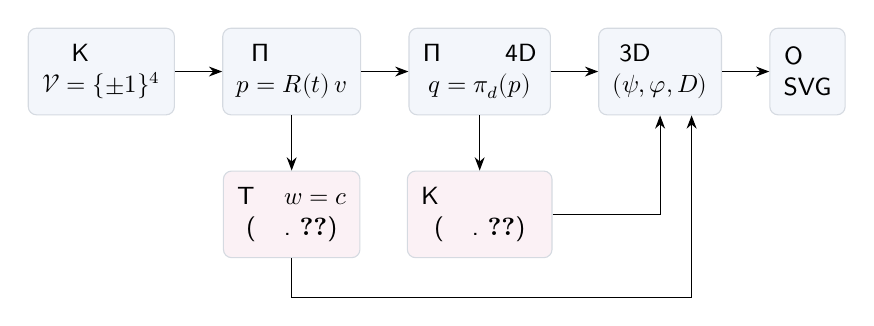
\begin{tikzpicture}[node distance=7mm and 6mm, box/.style={draw=rule,fill=accentA!6,rounded corners=3pt,align=center,font=\sffamily\small,inner sep=5pt,minimum height=11mm}, >=Stealth]
\node[box] (V) {Κορυφές\\$\V=\{\pm1\}^4$};
\node[box,right=of V] (R) {Περιστροφή\\$p=R(t)\,v$};
\node[box,right=of R] (P) {Προοπτική 4D\\$q=\pi_d(p)$};
\node[box,right=of P] (K) {3D κάμερα\\$(\psi,\varphi,D)$};
\node[box,right=of K] (S) {Οθόνη\\SVG};
\node[box,fill=accentB!8,below=of P] (H) {Κυρτό περίβλημα\\(ενότ.~\ref{sec:hull})};
\node[box,fill=accentB!8,below=of R] (T) {Τομή $w=c$\\(ενότ.~\ref{sec:slice})};
\draw[->] (V)--(R); \draw[->] (R)--(P); \draw[->] (P)--(K); \draw[->] (K)--(S);
\draw[->] (P)--(H); \draw[->] (R)--(T);
\draw[->] (H.east) -| (K.south);
\draw[->] (T.south) |- ++(0,-5mm) -| ($(K.south)+(4mm,0)$);
\end{tikzpicture}
\caption{Η ροή των υπολογισμών σε κάθε καρέ. Η τομή δεν περνά από την 4D προοπτική, γιατί βρίσκεται ήδη μέσα σε έναν τρισδιάστατο χώρο.}
\label{fig:pipeline}
\end{figure}

\paragraph{Συμβολισμοί} Γράφουμε τα σημεία του $\R^4$ ως $p=(p_x,p_y,p_z,p_w)$ και $\bar p=(p_x,p_y,p_z)$ για τις τρεις πρώτες συντεταγμένες. Με $e_1,\dots,e_4$ συμβολίζουμε την κανονική βάση και με $\langle\cdot,\cdot\rangle$ ή «$\cdot$» το ευκλείδειο εσωτερικό γινόμενο. Οι γωνίες των ρυθμιστών είναι σε μοίρες. Στους τύπους χρησιμοποιούνται ακτίνια.

%=====================================================================
\section{Ο υπερκύβος}
\begin{definition}
Ο (στερεός) υπερκύβος είναι το $\C=[-1,1]^4=\{x\in\R^4:\ |x_k|\le1,\ k=1,\dots,4\}$. Οι κορυφές του αριθμούνται με $i=0,\dots,15$:
\[
v_i=\bigl(2b_0(i)-1,\;2b_1(i)-1,\;2b_2(i)-1,\;2b_3(i)-1\bigr),\qquad b_k(i)=\lfloor i/2^k\rfloor \bmod 2 .
\]
Δύο κορυφές $v_i,v_j$ συνδέονται με ακμή αν και μόνο αν διαφέρουν σε ακριβώς μία συντεταγμένη, δηλαδή αν $i\oplus j=2^k$ (XOR). Ο δείκτης $k$ είναι ο \emph{άξονας} της ακμής.
\end{definition}
Ο κώδικας κατασκευάζει ακριβώς αυτές τις λίστες (\code{vertices}, \code{edges}).

\begin{proposition}\label{prop:fvector}
Το $\C$ έχει $f$-διάνυσμα $(f_0,f_1,f_2,f_3)=(16,32,24,8)$: 16 κορυφές, 32 ακμές, 24 τετράγωνες έδρες και 8 κυβικά κελιά. Ισχύει $f_0-f_1+f_2-f_3=0$ (Euler–Poincaré σε διάσταση 4). Επιπλέον $\|v_i\|=2$ για κάθε κορυφή.
\end{proposition}
\begin{proof}
Μια $j$-διάστατη έδρα προκύπτει αν επιλέξουμε $j$ «ελεύθερες» συντεταγμένες και δώσουμε τιμή $\pm1$ στις υπόλοιπες $4-j$. Άρα $f_j=\binom{4}{j}2^{4-j}$, που δίνει $16,32,24,8$. Τέλος, $\|v_i\|^2=4\cdot1=4$.
\end{proof}

\begin{definition}
Για $k\in\{1,2,3,4\}$ και $s\in\{-1,+1\}$, το \emph{κελί} $X_k^s=\{x\in\C:\ x_k=s\}$ είναι κύβος με εξωτερικό κάθετο διάνυσμα $s\,e_k$. Συμβολίζουμε τα κελιά με X$\pm$, Y$\pm$, Z$\pm$, W$\pm$.
\end{definition}
Δύο κελιά σε \emph{διαφορετικούς} άξονες έχουν ως κοινή έδρα ακριβώς ένα τετράγωνο. Τα δύο κελιά του ίδιου άξονα είναι ξένα μεταξύ τους. Κάθε τετράγωνο ανήκει σε ακριβώς δύο κελιά. Οι παρατηρήσεις αυτές χρησιμοποιούνται στο Θεώρημα~\ref{thm:cells}.

%=====================================================================
\section{Περιστροφές στον \texorpdfstring{$\R^4$}{R4}}
\begin{definition}
Για δύο άξονες $a\neq b$ και γωνία $\theta$, η στοιχειώδης στροφή (στροφή \eng{Givens}) στο επίπεδο $ab$ είναι η γραμμική απεικόνιση
\[
\bigl(R_{ab}(\theta)\,p\bigr)_a=\cos\theta\,p_a-\sin\theta\,p_b,\qquad
\bigl(R_{ab}(\theta)\,p\bigr)_b=\sin\theta\,p_a+\cos\theta\,p_b,
\]
που αφήνει αμετάβλητες τις άλλες δύο συντεταγμένες. Ο πίνακάς της είναι ορθογώνιος με ορίζουσα $1$. Επομένως $R_{ab}(\theta)\in SO(4)$.
\end{definition}
Στον $\R^4$ μια στοιχειώδης στροφή δεν γίνεται γύρω από άξονα. Γίνεται \emph{μέσα σε ένα επίπεδο} και αφήνει σταθερό ένα ολόκληρο συμπληρωματικό επίπεδο. Υπάρχουν $\binom42=6$ επίπεδα συντεταγμένων: $XY, XZ, XW, YZ, YW, ZW$. Οι στροφές $XW$, $YW$, $ZW$ αναμειγνύουν τη συντεταγμένη $w$ με τις ορατές συντεταγμένες. Γι' αυτό αλλάζουν το σχήμα της προβολής.

\paragraph{Η περιστροφή της εφαρμογής} Με $\theta_{xw},\theta_{yw},\theta_{zw}$ τις τιμές των ρυθμιστών και $t$ τον χρόνο της αυτόματης περιστροφής σε δευτερόλεπτα (\code{phase}), η συνάρτηση \code{rotate4} υπολογίζει
\begin{equation}\label{eq:R}
R(t)=R_{xy}(0.12\,t)\;R_{zw}(\theta_{zw})\;R_{yw}\!\bigl(\theta_{yw}+17^\circ t\bigr)\;R_{xw}\!\bigl(\theta_{xw}+27^\circ t\bigr),
\end{equation}
δηλαδή εφαρμόζει πρώτα τη στροφή $XW$, μετά τη $YW$, μετά τη $ZW$ και τελευταία την $XY$. Οι στροφές του $\R^4$ \emph{δεν} αντιμετατίθενται, άρα η σειρά έχει σημασία. Η σειρά $XW\to YW\to ZW$ και η σύμβαση πρόσημου είναι ίδιες με του \eng{Tesseract Explorer} (ενότητα~\ref{sec:verify}). Όταν η αυτόματη περιστροφή είναι σβηστή και $t=0$, ισχύει $R=R_{zw}R_{yw}R_{xw}$. Το κουμπί «Δείξε 3D κύβο» δίνει $R=I$.

\begin{lemma}\label{lem:wbound}
Για κάθε στροφή $R$ και κάθε κορυφή ισχύει $|(Rv_i)_w|\le\|Rv_i\|=2$. Επιπλέον
\[
W_{\max}:=\max_i|(Rv_i)_w|=\|\rho\|_1\in[1,2],
\]
όπου $\rho$ είναι η τέταρτη γραμμή του $R$.
\end{lemma}
\begin{proof}
Η $R$ διατηρεί τα μήκη, άρα $\|Rv_i\|=2$. Επίσης $(Rv)_w=\rho\cdot v$, και η μέγιστη τιμή μιας γραμμικής συνάρτησης πάνω στο $\{\pm1\}^4$ είναι $\|\rho\|_1$. Αφού $\|\rho\|_2=1$, παίρνουμε $1\le\|\rho\|_1\le\sqrt4\,\|\rho\|_2=2$.
\end{proof}

%=====================================================================
\section{Προοπτική προβολή \texorpdfstring{$4\mathrm{D}\to3\mathrm{D}$}{4D→3D}}\label{sec:persp}
Τοποθετούμε μια «4D κάμερα» στο σημείο $E_4=(0,0,0,d)$ και ως «φιλμ» παίρνουμε το υπερεπίπεδο $w=0$. Ο ρυθμιστής «4D προοπτική» δίνει την τιμή του $d\in[2.6,\,8]$, με προεπιλογή $3.8$.

\begin{definition}
Η προοπτική προβολή από το $E_4$ στο $\{w=0\}\cong\R^3$ είναι
\begin{equation}\label{eq:pi}
\pi_d(p)=\frac{d}{d-p_w}\,\bar p .
\end{equation}
\end{definition}
\begin{proof}[Παραγωγή]
Η ευθεία από το $E_4$ προς το $p$ γράφεται $E_4+s(p-E_4)$. Η συντεταγμένη $w$ μηδενίζεται όταν $d+s(p_w-d)=0$, δηλαδή όταν $s=d/(d-p_w)$. Τότε οι τρεις πρώτες συντεταγμένες είναι $s\,\bar p$ (σχήμα~\ref{fig:persp}).
\end{proof}

\begin{figure}[h]
\centering
\begin{tikzpicture}[scale=1.05,>=Stealth]
\draw[->,muted] (-0.3,0)--(5.4,0) node[right,font=\small]{$\|\bar p\|$};
\draw[->,muted] (0,-0.4)--(0,4.2) node[above,font=\small]{$w$};
\fill[accentB] (0,3.6) circle(2pt) node[left,font=\small]{$E_4=(0,d)$};
\fill[accentA] (1.6,1.2) circle(2pt) node[right=2pt,font=\small]{$p=(\|\bar p\|,p_w)$};
\draw[accentB,thick] (0,3.6)--(2.4,0);
\fill[accentB] (2.4,0) circle(2pt) node[below,font=\small]{$\dfrac{d}{d-p_w}\|\bar p\|$};
\draw[dashed,muted] (1.6,1.2)--(1.6,0) node[below,font=\small]{$\|\bar p\|$};
\draw[dashed,muted] (0,1.2)--(1.6,1.2);
\node[left,font=\small] at (0,1.2){$p_w$};
\node[font=\small,muted] at (4.3,0.35){φιλμ $w=0$};
\end{tikzpicture}
\caption{Όμοια τρίγωνα: $\dfrac{\|\pi_d(p)\|}{d}=\dfrac{\|\bar p\|}{d-p_w}$.}
\label{fig:persp}
\end{figure}

\begin{lemma}\label{lem:welldef}
Για κάθε $d\ge2.6$ και κάθε περιστραμμένο σημείο του $\C$ ο παρονομαστής είναι θετικός. Πιο συγκεκριμένα $d-p_w\ge d-2>0$, και ο συντελεστής κλίμακας $\kappa_4=d/(d-p_w)$ βρίσκεται στο διάστημα $\bigl[\tfrac{d}{d+2},\tfrac{d}{d-2}\bigr]$.
\end{lemma}
\begin{proof}
Από το Λήμμα~\ref{lem:wbound}, $|p_w|\le\|p\|\le2$ για κάθε $p\in R\C$, αφού $\C$ περιέχεται στη σφαίρα ακτίνας 2.
\end{proof}

\begin{proposition}[φράγμα μεγέθους]\label{prop:size}
Για $d>2$ ισχύει
\[
\max_{\|v\|=2}\|\pi_d(v)\|=\frac{2d}{\sqrt{d^2-4}},
\]
και το μέγιστο επιτυγχάνεται όταν $v_w=4/d$. Για $d=2.6,\ 3.8,\ 8$ το μέγιστο είναι αντίστοιχα $3.130,\ 2.352,\ 2.066$.
\end{proposition}
\begin{proof}
Θέτουμε $v_w=\omega$ και $\|\bar v\|=\sqrt{4-\omega^2}$. Τότε $f(\omega)=d\sqrt{4-\omega^2}/(d-\omega)$ και
\[
(\ln f)'=-\frac{\omega}{4-\omega^2}+\frac{1}{d-\omega}=0\iff 4-\omega^2=\omega d-\omega^2\iff \omega=\tfrac4d .
\]
Με αντικατάσταση: $f(4/d)=d\cdot\frac2d\sqrt{d^2-4}\cdot\frac{d}{d^2-4}=\frac{2d}{\sqrt{d^2-4}}$. Τα αριθμητικά δεδομένα ελέγχθηκαν και με πλήρη σάρωση.
\end{proof}
Το φράγμα αυτό χρειάζεται στην ενότητα~\ref{sec:camera}: όλα τα σημεία του $\R^3$ έχουν μέτρο το πολύ $3.13<5$, άρα η 3D κάμερα δεν «περνά ποτέ μέσα» από το σχήμα.

\begin{example}[κύβος μέσα σε κύβο]
Για $R=I$ το κελί $X_4^{+}$ (όπου $w=+1$) απεικονίζεται σε κύβο με ημιπλευρά $d/(d-1)$, και το κελί $X_4^{-}$ σε κύβο με ημιπλευρά $d/(d+1)$. Για $d=3.8$ οι τιμές είναι $1.357$ και $0.792$, με λόγο $(d+1)/(d-1)\approx1.714$. Αυτή είναι η γνωστή εικόνα «κύβος μέσα σε κύβο».
\end{example}

\begin{remark}[ορθογραφικό όριο]
Όταν $d\to\infty$, ο συντελεστής $\kappa_4\to1$ και η $\pi_d$ τείνει στην ορθογραφική προβολή $p\mapsto\bar p$. Μεγάλες τιμές του ρυθμιστή δίνουν ουσιαστικά ορθογραφική εικόνα.
\end{remark}

\paragraph{Σχέση με το \eng{Tesseract Explorer}} Εκεί χρησιμοποιείται $x'=f\,x/(c-w)$ με $f=2$ και $c=3$. Για $d=3$, ο τύπος~\eqref{eq:pi} δίνει ακριβώς $\tfrac{3}{2}$ φορές το ίδιο σημείο, δηλαδή ομοιόμορφη κλιμάκωση. Το σχήμα είναι επομένως το ίδιο (αριθμητικός έλεγχος στην ενότητα~\ref{sec:verify}).

%=====================================================================
\section{Το θεώρημα κυρτότητας}
Το επόμενο αποτέλεσμα δικαιολογεί γιατί η δεξιά όψη υπολογίζει \emph{κυρτό περίβλημα}.

\begin{lemma}[κυρτοί συνδυασμοί]\label{lem:combo}
Έστω $u_1,\dots,u_m\in\R^4$ με $(u_i)_w<d$ και βάρη $\lambda_i\ge0$ με $\sum\lambda_i=1$. Τότε
\[
\pi_d\Bigl(\sum_i\lambda_iu_i\Bigr)=\sum_i\mu_i\,\pi_d(u_i),\qquad
\mu_i=\frac{\lambda_i\,(d-(u_i)_w)}{\sum_j\lambda_j\,(d-(u_j)_w)}\ \ge0,\quad \sum_i\mu_i=1 .
\]
\end{lemma}
\begin{proof}
Θέτουμε $\Delta=\sum_j\lambda_j(d-(u_j)_w)=d-\bigl(\sum_j\lambda_ju_j\bigr)_w>0$. Τότε
\[
\sum_i\mu_i\,\pi_d(u_i)=\sum_i\frac{\lambda_i(d-(u_i)_w)}{\Delta}\cdot\frac{d\,\bar u_i}{d-(u_i)_w}
=\frac{d}{\Delta}\sum_i\lambda_i\bar u_i=\pi_d\Bigl(\sum_i\lambda_iu_i\Bigr). \qedhere
\]
\end{proof}
Για $m=2$ το λήμμα λέει ότι η εικόνα του ευθύγραμμου τμήματος $[a,b]$ είναι το τμήμα $[\pi_d(a),\pi_d(b)]$. Η παράμετρος αλλάζει με αύξουσα συνάρτηση \eng{Möbius}:
\begin{equation}\label{eq:mobius}
\pi_d\bigl((1-t)a+tb\bigr)=(1-\sigma)\pi_d(a)+\sigma\pi_d(b),\qquad
\sigma(t)=\frac{t\,(d-b_w)}{(1-t)(d-a_w)+t\,(d-b_w)} .
\end{equation}

\begin{theorem}\label{thm:convex}
Για κάθε στροφή $R$ και κάθε $d>2$ ισχύει
\[
\pi_d(R\,\C)=\conv\{\pi_d(Rv_i):\ i=0,\dots,15\}.
\]
Με άλλα λόγια, η 3D «σκιά» του στερεού υπερκύβου είναι το κυρτό περίβλημα των 16 προβαλλόμενων κορυφών.
\end{theorem}
\begin{proof}
($\subseteq$) Κάθε $x\in R\C$ γράφεται ως κυρτός συνδυασμός των κορυφών $Rv_i$. Από το Λήμμα~\ref{lem:combo}, το $\pi_d(x)$ είναι κυρτός συνδυασμός των $\pi_d(Rv_i)$. Η υπόθεση $(u_i)_w<d$ ισχύει από το Λήμμα~\ref{lem:welldef}.
($\supseteq$) Έστω $y=\sum\mu_i\pi_d(Rv_i)$ με $\mu_i\ge0$ και $\sum\mu_i=1$. Λύνουμε ως προς $\lambda$ τη σχέση του λήμματος: θέτουμε $\lambda_i\propto\mu_i/(d-(Rv_i)_w)$ και κανονικοποιούμε. Αυτό δίνει θετικά βάρη, και τότε $y=\pi_d\bigl(\sum\lambda_iRv_i\bigr)\in\pi_d(R\C)$.
\end{proof}

\begin{corollary}
Η όψη «Προβολή · περίβλημα» δείχνει ακριβώς ό,τι δείχνει η αδιαφανής απόδοση (\eng{solid}) του \eng{Tesseract Explorer}. Εκεί τα 8 προβαλλόμενα κελιά σχεδιάζονται αδιαφανή με έλεγχο βάθους. Η εξωτερική επιφάνεια της ένωσής τους είναι το σύνορο του $\pi_d(R\C)$ (σχήμα~\ref{fig:compare}).
\end{corollary}

%=====================================================================
\section{Υπολογισμός του κυρτού περιβλήματος}\label{sec:hull}
Θέτουμε $q_i=\pi_d(Rv_i)\in\R^3$ για $i=0,\dots,15$. Η συνάρτηση \code{hull3D} εφαρμόζει τον εξής αλγόριθμο εξαντλητικής αναζήτησης, με ανοχή $\varepsilon=10^{-7}$:

\begin{enumerate}[label=\arabic*.]
\item Για κάθε τριάδα $i<j<k$ (συνολικά $\binom{16}{3}=560$) υπολόγισε $n=(q_j-q_i)\times(q_k-q_i)$. Αν $\|n\|<\varepsilon$ τα σημεία είναι συνευθειακά και η τριάδα παραλείπεται. Αλλιώς κανονικοποίησε το $n$.
\item Υπολόγισε τις αποστάσεις $\delta_m=n\cdot(q_m-q_i)$ για όλα τα $m$. Αν υπάρχουν και θετικές και αρνητικές (πέρα από το $\varepsilon$), το επίπεδο τέμνει το σχήμα και η τριάδα απορρίπτεται.
\item Προσανατόλισε το $n$ ώστε να ισχύει $\delta_m\le\varepsilon$ για όλα τα $m$, δηλαδή ώστε να είναι \emph{εξωτερικό} κάθετο.
\item Η έδρα είναι το σύνολο $F=\{m:\ |n\cdot q_m-n\cdot q_i|<\varepsilon\}$. Οι διπλές εμφανίσεις (ίδιο $F$) αγνοούνται.
\item Ταξινόμησε τις κορυφές του $F$ κατά γωνία γύρω από το κέντρο βάρους. Η γωνία μετριέται ως $\operatorname{atan2}(\delta\cdot v,\delta\cdot u)$ στη βάση $u=r\times n$, $v=n\times u$ του επιπέδου, όπου $r=e_3$ ή $e_2$.
\end{enumerate}

\begin{lemma}[ορθότητα]
Ένα επίπεδο $H$ ορίζει έδρα (2-διάστατη) ενός κυρτού πολυέδρου $P=\conv Q$ αν και μόνο αν (α) περιέχει τρία μη συνευθειακά σημεία του $Q$ και (β) όλο το $Q$ βρίσκεται στον ίδιο κλειστό ημιχώρο του $H$. Τότε η έδρα είναι $\conv(Q\cap H)$.
\end{lemma}
\begin{proof}
Αν το $H$ στηρίζει το $P$ και το $H\cap P$ έχει διάσταση 2, τότε το $H\cap P$ είναι πολύγωνο με κορυφές στο $Q$. Επομένως περιέχει τρεις μη συνευθειακές κορυφές. Αντίστροφα, το (β) σημαίνει ότι το $H$ στηρίζει το $P$. Το (α) εξασφαλίζει ότι $\dim(H\cap P)=2$. Επιπλέον $H\cap P=H\cap\conv Q=\conv(Q\cap H)$, αφού όλα τα σημεία του $Q$ βρίσκονται από τη μία πλευρά του $H$.
\end{proof}
Ο αλγόριθμος απαριθμεί επομένως ακριβώς τις έδρες. Το κόστος είναι $560\times16\approx9\,000$ εσωτερικά γινόμενα ανά καρέ, αμελητέο για 16 σημεία. Για πολλά σημεία θα χρειαζόταν ο αλγόριθμος \eng{Quickhull}~\cite{quickhull}.

%=====================================================================
\section{Πόσες έδρες έχει η προβολή: το θεώρημα ορατών κελιών}
Στα πειράματα η δεξιά όψη εμφανίζει μόνο τρεις συνδυασμούς: 6, 10 ή 12 έδρες, με 8, 12 ή 14 κορυφές αντίστοιχα. Το παρακάτω θεώρημα εξηγεί γιατί.

\begin{definition}
Έστω $c=R^{\top}E_4=d\,R^{\top}e_4$ η θέση της 4D κάμερας στο σύστημα συντεταγμένων του ίδιου του υπερκύβου. Το κελί $X_k^s$ λέγεται \emph{ορατό} αν $s\,c_k>1$, δηλαδή αν η κάμερα βρίσκεται στην εξωτερική πλευρά του υπερεπιπέδου $x_k=s$. Ορίζουμε $k_{\mathrm{vis}}=\#\{k:\ |c_k|>1\}$.
\end{definition}
Ισχύει πάντα $1\le k_{\mathrm{vis}}\le4$, γιατί $\|c\|=d>2$, άρα $\max_k|c_k|\ge d/2>1$. Για κάθε άξονα το πολύ ένα από τα δύο κελιά του είναι ορατό.

\begin{theorem}\label{thm:cells}
Αν κανένα $|c_k|$ δεν είναι ίσο με 1 (γενική θέση), τότε το πολύεδρο $\pi_d(R\C)$ έχει
\[
F=k_{\mathrm{vis}}\,(7-k_{\mathrm{vis}}),\qquad E=2F,\qquad V=F+2,
\]
δηλαδή $(V,E,F)=(8,12,6),\,(12,20,10),\,(14,24,12),\,(14,24,12)$ για $k_{\mathrm{vis}}=1,2,3,4$.
\end{theorem}
\begin{proof}[Σκιαγράφηση απόδειξης]
Όπως όταν ένας 3D κύβος φωτίζεται από σημειακή πηγή, το σύνορο της σκιάς ενός κυρτού πολυτόπου $P$ από σημείο $E\notin P$ αποτελείται από τις εικόνες των \emph{περιγραμμικών} έδρων διάστασης $\dim P-2$. Αυτές είναι οι έδρες που ανήκουν ταυτόχρονα σε μία ορατή και σε μία μη ορατή έδρα μέγιστης διάστασης (\eng{shadow boundary}, βλ.~\cite{ziegler}). Για τον υπερκύβο, οι έδρες μέγιστης διάστασης είναι τα κελιά και οι περιγραμμικές έδρες είναι τετράγωνα. Το κελί $X_k^s$ έχει εξωτερικό κάθετο $R(se_k)$ και στηρικτικό υπερεπίπεδο $\{p:\ R(se_k)\cdot p=1\}$. Το $E_4$ βρίσκεται στην εξωτερική του πλευρά ακριβώς όταν $s\,(R^\top E_4)_k=s\,c_k>1$.

Μένει να μετρήσουμε τα ζεύγη (ορατό, μη ορατό) κελιών σε διαφορετικούς άξονες, αφού κάθε τέτοιο ζεύγος μοιράζεται ένα τετράγωνο. Ένα ορατό κελί στον άξονα $i$ γειτονεύει με $1$ μη ορατό κελί σε καθέναν από τους άλλους $k_{\mathrm{vis}}-1$ «ορατούς» άξονες και με $2$ μη ορατά κελιά σε καθέναν από τους $4-k_{\mathrm{vis}}$ υπόλοιπους. Άρα $F=k_{\mathrm{vis}}\bigl[(k_{\mathrm{vis}}-1)+2(4-k_{\mathrm{vis}})\bigr]=k_{\mathrm{vis}}(7-k_{\mathrm{vis}})$. Η προβολή στέλνει τετράγωνα σε τετράπλευρα. Κάθε ακμή ανήκει σε δύο έδρες, άρα $E=4F/2=2F$, και από τον τύπο του Euler $V-E+F=2$ προκύπτει $V=F+2$.
\end{proof}

\begin{remark}
(α) Για $R=I$ έχουμε $c=(0,0,0,d)$, άρα $k_{\mathrm{vis}}=1$, και η εικόνα είναι κύβος με 6 έδρες. Αυτό κάνει το κουμπί «Δείξε 3D κύβο».
(β) Στο ορθογραφικό όριο $d\to\infty$ μετράει μόνο η διεύθυνση του $c$. Γενικά $k_{\mathrm{vis}}=4$, άρα προκύπτει πολύεδρο με 14 κορυφές και 12 έδρες. Αυτό συμφωνεί με το αποτέλεσμα του \eng{Finch} για τυχαίες ορθογώνιες προβολές τάξης 3~\cite{finch}.
(γ) Αριθμητικός έλεγχος σε 20\,000 τυχαίες καταστάσεις: ο τύπος επαληθεύτηκε σε όλες. Η κατανομή ήταν $k_{\mathrm{vis}}=1,2,3,4$ σε $3785,\,6348,\,6345,\,3522$ καταστάσεις αντίστοιχα.
\end{remark}

%=====================================================================
\section{Από τον \texorpdfstring{$\R^3$}{R3} στην οθόνη}\label{sec:camera}
\paragraph{Κάμερα} Η συνάρτηση \code{camera} περιστρέφει πρώτα κατά γωνία $\psi$ (\eng{yaw}) γύρω από τον άξονα $y$ και μετά κατά γωνία $\varphi$ (\eng{pitch}) γύρω από τον άξονα $x$:
\[
\begin{aligned}
x' &= \cos\psi\,x+\sin\psi\,z, & z' &= -\sin\psi\,x+\cos\psi\,z,\\
x_c&=x', & y_c&=\cos\varphi\,y-\sin\varphi\,z',\qquad z_c=\sin\varphi\,y+\cos\varphi\,z'.
\end{aligned}
\]
Το σύρσιμο με το ποντίκι αλλάζει το $\psi$ κατά $0.009$ ακτίνια ανά pixel. Το $\varphi$ αλλάζει με τον ίδιο ρυθμό και περιορίζεται στο $[-1.45,1.45]$.

\paragraph{3D προοπτική και οθόνη} Το μάτι βρίσκεται στο $(0,0,D)$ με $D=5$ (σταθερά \code{EYE}). Με $\kappa_3=D/(D-z_c)$ και μεγέθυνση $\zeta$:
\[
x_s=250+69\,\zeta\,\kappa_3\,x_c,\qquad y_s=220-69\,\zeta\,\kappa_3\,y_c .
\]
Από την Πρόταση~\ref{prop:size} ισχύει $|z_c|\le\|q\|\le3.13<D$, άρα $\kappa_3\in(0.61,\,2.7)$ και η εικόνα είναι πάντα καλά ορισμένη. Η \code{fitPoints} εφαρμόζει στο τέλος έναν \emph{μετασχηματισμό ομοιότητας}: κεντράρει την εικόνα και πολλαπλασιάζει με $\sigma=\min\bigl(1,\ 440/\Delta x,\ 365/\Delta y\bigr)$. Έτσι το σχήμα χωράει στο πλαίσιο χωρίς παραμόρφωση. Το $\sigma\le1$, άρα η εικόνα μόνο σμικρύνεται.

\paragraph{Ορατότητα έδρας} Μια έδρα με εξωτερικό κάθετο $n$ και κέντρο $m$ (σε συντεταγμένες κάμερας) είναι ορατή αν και μόνο αν
\begin{equation}\label{eq:visible}
n\cdot\bigl((0,0,D)-m\bigr)>0 .
\end{equation}
Η εφαρμογή (συνάρτηση \code{facing}) χρησιμοποιεί την κανονικοποιημένη ποσότητα $f=n\cdot(E-m)/\bigl(\|n\|\,\|E-m\|\bigr)\in[-1,1]$, που είναι το συνημίτονο της γωνίας θέασης. Η v1 χρησιμοποιούσε το κριτήριο $n_z>0$, που ισχύει μόνο για ορθογραφική κάμερα ($D\to\infty$). Με την πραγματική κάμερα ($D=5$) το κριτήριο αυτό χαρακτήριζε λάθος περίπου 4\,000 έδρες σε 3\,000 τυχαίες καταστάσεις, σε περίπου 3 στις 4 καταστάσεις. Το αποτέλεσμα ήταν να φαίνονται πίσω κορυφές και ακμές «μέσα» από το στερεό. Με το~\eqref{eq:visible} τα λάθη είναι 0.

\begin{lemma}
Για κυρτό πολύεδρο και μάτι εκτός αυτού, οι εικόνες των ορατών εδρών δεν επικαλύπτονται και καλύπτουν όλη την εικόνα του πολυέδρου.
\end{lemma}
\begin{proof}
Μια ακτίνα από το μάτι που συναντά το κυρτό σώμα μπαίνει σε αυτό σε ακριβώς ένα σημείο του συνόρου. Το σημείο αυτό ανήκει σε ορατή έδρα, και η ακτίνα δεν συναντά άλλη ορατή έδρα πριν βγει από το σώμα.
\end{proof}
Γι' αυτό η σειρά σχεδίασης δεν επηρεάζει τις ορατές έδρες της προβολής. Η εφαρμογή ταξινομεί πάντως κατά $z_c$ (αλγόριθμος του ζωγράφου), γιατί στην τομή σχεδιάζονται και οι πίσω έδρες με χαμηλή αδιαφάνεια.

\paragraph{Σκίαση} Ο φωτισμός μιας έδρας είναι $L=\max\bigl(0,\ \hat n\cdot(0.3,\,0.6,\,0.7)\bigr)$. Η αδιαφάνεια της έδρας είναι $\alpha=\min(0.94,\ 0.66+0.22L+0.08f)$ στην προβολή και $\alpha=\min(0.70,\ 0.24+0.28L+0.14f)$ στην τομή. Οι πίσω έδρες της τομής έχουν $\alpha=0.045$. Στον σκελετό, η διαφάνεια μιας ακμής εξαρτάται από το βάθος $\bar z$: $\alpha=\operatorname{clamp}(0.65+0.11\bar z,\ 0.34,\ 0.98)$.

%=====================================================================
\section{Τομή με υπερεπίπεδο \texorpdfstring{$W=c$}{W=c}}\label{sec:slice}
\begin{definition}
Για $c\in\R$, η τομή είναι $S_c=\{\bar p:\ p\in R\C,\ p_w=c\}\subset\R^3$. Με $a_k=Re_k$ (η $k$-οστή στήλη του $R$) ισχύει η αναπαράσταση με ημιχώρους
\[
S_c=\Bigl\{x\in\R^3:\ \bigl|a_k\cdot(x,c)\bigr|\le1,\ k=1,\dots,4\Bigr\}.
\]
\end{definition}
Πράγματι, οι αρχικές συντεταγμένες του $p$ είναι $R^\top p$, με $k$-οστή συντεταγμένη $a_k\cdot p$. Το $S_c$ είναι μη κενό αν και μόνο αν $|c|\le W_{\max}$ (Λήμμα~\ref{lem:wbound}). Αφού $W_{\max}\ge1$ και ο ρυθμιστής περιορίζεται στο $|c|\le0.85$, η τομή είναι πάντα πραγματικό τρισδιάστατο πολύεδρο.

\begin{theorem}\label{thm:slicevert}
Οι κορυφές του $S_c$ είναι ακριβώς τα σημεία όπου το υπερεπίπεδο $\{p_w=c\}$ συναντά τις ακμές του $R\C$, συμπεριλαμβανομένων των κορυφών του $R\C$ που ανήκουν σε αυτό.
\end{theorem}
\begin{proof}
Έστω $x$ κορυφή του $P\cap H$, όπου $P=R\C$ και $H=\{p_w=c\}$. Έστω $G$ η ελάχιστη έδρα του $P$ που περιέχει το $x$, οπότε $x\in\relint G$. Αν $\dim G\ge2$, τότε το $\aff G\cap H$ έχει διάσταση τουλάχιστον 1 κοντά στο $x$. Επομένως το $x$ θα ήταν εσωτερικό σημείο ενός ευθύγραμμου τμήματος μέσα στο $P\cap H$, που είναι άτοπο για κορυφή. Άρα $\dim G\le1$, δηλαδή το $x$ είναι κορυφή του $P$ ή σημείο ακμής του.
\end{proof}
Για την ακμή $[a,b]$ με $a_w\neq b_w$, το σημείο τομής είναι
\[
t=\frac{c-a_w}{b_w-a_w}\in[0,1],\qquad x=\bar a+t\,(\bar b-\bar a).
\]
Ακμές με $a_w=b_w$ παραλείπονται. Αν τέτοια ακμή βρίσκεται μέσα στο $H$, τα άκρα της είναι κορυφές του $P$ και τα βρίσκουν οι γειτονικές ακμές. Πανομοιότυπα σημεία συγχωνεύονται με ανοχή $10^{-6}$.

\paragraph{Έδρες} Κάθε κελί $X_k^s$ που τέμνει το $H$ σε διάσταση 2 δίνει μία έδρα: το πολύγωνο που σχηματίζουν τα σημεία τομής των ακμών του κελιού. Το εξωτερικό κάθετο της έδρας μέσα στο $H\cong\R^3$ είναι το $\overline{s\,a_k}$ κανονικοποιημένο. Επομένως $F\le8$.

\begin{remark}[εκφυλισμένη περίπτωση, διορθώθηκε στη v3]
Όταν το $H$ περιέχει ολόκληρο ένα τετράγωνο $Q=X_k^s\cap X_l^t$ του υπερκύβου, \emph{και τα δύο} κελιά δίνουν το ίδιο πολύγωνο $Q$. Παράδειγμα: $XW=45^\circ$, $YW=ZW=0^\circ$, $c=0$. Η τομή είναι το ορθογώνιο κουτί $[-\sqrt2,\sqrt2]\times[-1,1]^2$ με 6 έδρες. Οι v1 και v2 μετρούσαν όμως 8 έδρες, με $V-E+F=4\neq2$, και σχεδίαζαν δύο φορές τις αντίστοιχες έδρες. Η v3 αφαιρεί τα διπλά πολύγωνα συγκρίνοντας τα σύνολα κορυφών τους. Σε σάρωση $546\,875$ καταστάσεων των ρυθμιστών (γωνίες ανά $15^\circ$, $c$ ανά $0.05$), η v2 αστόχησε σε 356 και η v3 σε καμία.
\end{remark}

\paragraph{Χαρακτηριστικά σχήματα}
\begin{itemize}
\item $R=I$ (\emph{κελί μπροστά}): για κάθε $|c|<1$ η τομή είναι ο κύβος $[-1,1]^3$.
\item Ειδικός προσανατολισμός με $W_{\max}=2$ (\emph{κορυφή μπροστά}): η τομή περνά από τετράεδρο σε κόλουρο τετράεδρο και γίνεται κανονικό οκτάεδρο στο $c=0$, με 6 κορυφές και 8 έδρες (σχήμα~\ref{fig:slices}).
\item Γενική θέση: πολύεδρα με έως 8 έδρες, για παράδειγμα με 12 κορυφές, 18 ακμές και 8 έδρες.
\end{itemize}
Η τομή σχεδιάζεται μόνο με την 3D κάμερα. Η 4D προοπτική δεν εφαρμόζεται, γιατί το $S_c$ βρίσκεται ήδη μέσα σε έναν τρισδιάστατο χώρο.

%=====================================================================
\section{Χρωματισμός και \eng{colormaps}}
\paragraph{Κανονικοποίηση του $W$} Σε κάθε καρέ υπολογίζεται το $W_{\max}=\max_i|(Rv_i)_w|\in[1,2]$ (Λήμμα~\ref{lem:wbound}) και η κανονικοποιημένη τιμή
\[
\tau(w)=\tfrac12\bigl(w/W_{\max}+1\bigr)\in[0,1].
\]
Η κανονικοποίηση είναι συμμετρική: το $w=0$ αντιστοιχεί πάντα στο μέσο $\tau=0.5$, που είναι το «ουδέτερο» χρώμα των αποκλινόντων \eng{colormaps} όπως το \eng{coolwarm}. Η $W_{\max}$ μεταβάλλεται συνεχώς με την περιστροφή, άρα και τα χρώματα αλλάζουν συνεχώς, χωρίς άλματα. Μεγαλύτερο $w$ σημαίνει πιο κοντά στην 4D κάμερα και μεγαλύτερη εικόνα, λόγω του $\kappa_4$.

\paragraph{Παρεμβολή} Κάθε \eng{colormap} αποθηκεύεται ως 11 δείγματα $s_0,\dots,s_{10}$ (sRGB) από το \eng{matplotlib}. Για τα \eng{inferno} και \eng{magma} τα δείγματα παίρνονται στο $[0.08,0.96]$, ώστε να αποφεύγεται το σχεδόν μαύρο και το σχεδόν λευκό. Το χρώμα υπολογίζεται τμηματικά γραμμικά:
\[
C(\tau)=(1-\phi)\,s_j+\phi\,s_{j+1},\qquad j=\min(9,\lfloor10\tau\rfloor),\quad \phi=10\tau-j .
\]
Η επιλογή «Αντιστροφή» αντικαθιστά το $\tau$ με $1-\tau$.

\paragraph{Τρόποι χρωματισμού}
\begin{itemize}
\item \emph{Σκελετός κατά $W$}: η κορυφή $i$ παίρνει το χρώμα $C(\tau(w_i))$. Κάθε ακμή είναι γραμμική διαβάθμιση SVG (\code{linearGradient} σε συντεταγμένες οθόνης) από το χρώμα της μίας κορυφής στο χρώμα της άλλης. Τα άκρα είναι ακριβή. Ενδιάμεσα, η παράμετρος οθόνης συνδέεται με την παράμετρο του $\R^4$ μέσω της αύξουσας συνάρτησης \eng{Möbius}~\eqref{eq:mobius} και της 3D προοπτικής. Η γραμμική διαβάθμιση στην οθόνη είναι επομένως προσέγγιση, πολύ καλή όταν $|b_w-a_w|\ll d$.
\item \emph{Σκελετός κατά άξονα}: οι ακμές του άξονα $k\in\{0,1,2,3\}$ (X, Y, Z, W) παίρνουν το χρώμα $C\bigl((k+\tfrac12)/4\bigr)$, δηλαδή τα κέντρα τεσσάρων ίσων διαστημάτων, μακριά από τα σκούρα άκρα.
\item \emph{Προβολή με \eng{colormap}}: η έδρα $F$ παίρνει το χρώμα $C(\tau(\bar w_F))$, όπου $\bar w_F$ είναι ο μέσος όρος του $w$ των κορυφών της.
\item \emph{Τομή με \eng{colormap}}: η έδρα από το κελί $X_k^s$ παίρνει το χρώμα $C\bigl((j+\tfrac12)/8\bigr)$ με $j=2k+[s=+]$. Έτσι φαίνεται από ποιο από τα 8 κελιά προέρχεται κάθε έδρα.
\end{itemize}

\paragraph{Αναγνωσιμότητα} Η αντίθεση μεταξύ δύο χρωμάτων υπολογίζεται κατά \eng{WCAG}~\cite{wcag}: $(L_1+0.05)/(L_2+0.05)$, όπου $L$ η σχετική φωτεινότητα. Αν μια ακμή έχει αντίθεση $<2.2$ με το φόντο (για παράδειγμα κίτρινο σε λευκό ή σκούρο μωβ σε μαύρο), σχεδιάζεται κάτω της ένα πλαίσιο στο χρώμα του κειμένου με αδιαφάνεια $0.3$. Αλλιώς σχεδιάζεται ένα «κενό» στο χρώμα του φόντου, που δείχνει ποια ακμή περνά μπροστά από ποια στις διασταυρώσεις.

\paragraph{Επιλογή \eng{colormap}} Τα \eng{viridis}, \eng{plasma}, \eng{inferno} και \eng{magma} είναι αντιληπτικά ομοιόμορφα~\cite{viridis}. Το \eng{cividis} είναι βελτιστοποιημένο για ελλείψεις στην αντίληψη χρωμάτων~\cite{cividis}. Το \eng{turbo} έχει μέγιστη αντίθεση αλλά δεν είναι ομοιόμορφο~\cite{turbo}. Το \eng{coolwarm} είναι αποκλίνον~\cite{moreland} και κατάλληλο για το πρόσημο του $W$.

\begin{figure}[p]
\centering
\includegraphics[width=.86\linewidth]{fig/cube.jpg}\par\smallskip
{\small (α) $R=I$: «κύβος μέσα σε κύβο» αριστερά, κύβος με 6 έδρες δεξιά ($k_{\mathrm{vis}}=1$).}\par\bigskip
\includegraphics[width=.86\linewidth]{fig/hull-wmap.jpg}\par\smallskip
{\small (β) Προεπιλεγμένες γωνίες, χρωματισμός κατά $W$ (\eng{viridis}): 14 κορυφές και 12 έδρες ($k_{\mathrm{vis}}\ge3$).}\par\bigskip
\includegraphics[width=.86\linewidth]{fig/hull-axis.jpg}\par\smallskip
{\small (γ) $XW=YW=ZW=45^\circ$, ακμές κατά άξονα (\eng{turbo}), έδρες κατά μέσο $W$.}
\caption{Προβολές από την εφαρμογή v3.}
\label{fig:proj}
\end{figure}

\begin{figure}[p]
\centering
\includegraphics[width=\linewidth]{fig/slice-cells.jpg}\par\smallskip
{\small (α) Τομή στο $c=0.2$ με τις προεπιλεγμένες γωνίες, κάθε έδρα χρωματισμένη κατά κελί.}\par\bigskip
\includegraphics[width=\linewidth]{fig/slice-octa.jpg}\par\smallskip
{\small (β) Προσανατολισμός «κορυφή μπροστά» ($W_{\max}=2$): στο $c=0$ η τομή είναι οκτάεδρο με 6 κορυφές και 8 έδρες, μία από κάθε κελί.}
\caption{Τομές από την εφαρμογή v3.}
\label{fig:slices}
\end{figure}

%=====================================================================
\section{Επαλήθευση}\label{sec:verify}
Όλοι οι έλεγχοι έγιναν πάνω στον ίδιο τον κώδικα του \code{index.html}: οι συναρτήσεις φορτώθηκαν απευθείας από το αρχείο, χωρίς αντιγραφή.

\begin{center}
\small
\begin{tabularx}{\linewidth}{@{}>{\raggedright\arraybackslash}p{4.3cm}>{\raggedright\arraybackslash}X>{\raggedright\arraybackslash}p{3.3cm}@{}}
\toprule
\textbf{Τι ελέγχθηκε} & \textbf{Μέθοδος} & \textbf{Αποτέλεσμα}\\
\midrule
Περιστροφές και 4D προοπτική & Σύγκριση με το \code{transform4D.js} του \eng{Tesseract Explorer} (ίδιες γωνίες, $d=3$, κλίμακα $3/2$), 2\,000 τυχαίες στροφές & μέγιστη απόκλιση $2.9\cdot10^{-7}$ (ακρίβεια \eng{float32})\\
Κυρτό περίβλημα & Σύγκριση με τη βιβλιοθήκη \eng{quickhull3d} (ένωση ομοεπίπεδων τριγώνων), 3\,000 τυχαίες καταστάσεις & ίδια σύνολα εδρών σε όλες\\
Ορατότητα εδρών & Ακριβές κριτήριο~\eqref{eq:visible} με ανεξάρτητα υπολογισμένα κάθετα & v1: $\approx4\,000$ λάθη· v3: 0\\
Θεώρημα~\ref{thm:cells} & $k_{\mathrm{vis}}$ από το $c=R^\top E_4$ έναντι των μετρημένων $(V,F)$, 20\,000 καταστάσεις & 100\,\% συμφωνία\\
Τομή & Ανεξάρτητη απαρίθμηση κορυφών της αναπαράστασης με ημιχώρους ($\binom83=56$ γραμμικά συστήματα $3\times3$), 3\,000 καταστάσεις, $c\in[-2,2]$ & ίδιες κορυφές και ίδιος αριθμός εδρών\\
Εκφυλισμένες τομές & Σάρωση $546\,875$ καταστάσεων των ρυθμιστών & v2: 356 λάθη· v3: 0\\
Τύπος του Euler & $V-E+F=2$ σε κάθε περίβλημα και κάθε τομή όλων των παραπάνω & ισχύει\\
Οπτική σύγκριση & Απόδοση \eng{solid/perspective} του \eng{Tesseract Explorer} και του περιβλήματος της v3, με ίδιες γωνίες και ίδια 3D κάμερα (σχήμα~\ref{fig:compare}) & ίδιο περίγραμμα\\
Περιηγητής & \eng{Chromium}: φωτεινό και σκοτεινό θέμα, πλάτος 390\,px, όλα τα κουμπιά & χωρίς σφάλματα, χωρίς οριζόντια κύλιση\\
\bottomrule
\end{tabularx}
\end{center}

\begin{figure}[h]
\centering
\includegraphics[width=\linewidth]{fig/compare.jpg}
\caption{Αριστερά σε κάθε ζεύγος: \eng{Tesseract Explorer} (αδιαφανής απόδοση, προοπτική, χρώματα κελιών του ίδιου του προγράμματος). Δεξιά: το περίβλημα της v3 με τις ίδιες γωνίες $(XW,YW,ZW)$ και την ίδια θέση 3D κάμερας. Οι γωνίες είναι $(0,0,0)$, $(38,22,12)$, $(45,45,45)$ και $(45,0,0)$ μοίρες. Το περίγραμμα συμπίπτει σε όλες τις περιπτώσεις.}
\label{fig:compare}
\end{figure}

%=====================================================================
\section{Αντιστοίχιση κώδικα και μαθηματικών}
\begin{center}
\small
\begin{tabularx}{\linewidth}{@{}>{\ttfamily}p{3.4cm}X@{}}
\toprule
\textrm{\textbf{Συνάρτηση}} & \textbf{Τι υπολογίζει}\\
\midrule
vertices, edges & $\V=\{\pm1\}^4$ με αρίθμηση bit, ακμές όταν $i\oplus j=2^k$\\
rotate, rotate4 & $R_{ab}(\theta)$ και η σύνθεση~\eqref{eq:R}\\
project4coords & $\pi_d(p)=\frac{d}{d-p_w}\bar p$, τύπος~\eqref{eq:pi}\\
camera, perspective & $\psi,\varphi$, $\kappa_3=D/(D-z_c)$, συντεταγμένες οθόνης\\
fitPoints & μετασχηματισμός ομοιότητας με $\sigma\le1$\\
hull3D & ο αλγόριθμος της ενότητας~\ref{sec:hull}, έδρες με μέσο $\bar w_F$\\
facing & κριτήριο ορατότητας~\eqref{eq:visible}, συνημίτονο $f$, φωτισμός $L$\\
crossSection & Θεώρημα~\ref{thm:slicevert}, έδρες ανά κελί, αφαίρεση διπλών εδρών\\
sampleStops & παρεμβολή $C(\tau)$\\
luminance, contrast & σχετική φωτεινότητα και λόγος αντίθεσης \eng{WCAG}\\
\bottomrule
\end{tabularx}
\end{center}

%=====================================================================
\begin{thebibliography}{99}\small
\bibitem{coxeter} H.\,S.\,M. Coxeter, \emph{\eng{Regular Polytopes}}, 3η έκδ., \eng{Dover}, 1973.
\bibitem{ziegler} G.\,M. Ziegler, \emph{\eng{Lectures on Polytopes}}, \eng{Graduate Texts in Mathematics} 152, \eng{Springer}, 1995.
\bibitem{hollasch} S.\,R. Hollasch, \emph{\eng{Four-Space Visualization of 4D Objects}}, μεταπτυχιακή εργασία, \eng{Arizona State University}, 1991.
\bibitem{finch} S.\,R. Finch, \emph{\eng{Rank-3 Projections of a 4-Cube}}, \eng{arXiv:1204.3468}, 2012.
\bibitem{sherif} T. Sherif, \emph{\eng{Tesseract Explorer}}, \url{https://github.com/tsherif/tesseract-explorer}, άδεια \eng{MIT}, 2020.
\bibitem{quickhull} C.\,B. Barber, D.\,P. Dobkin, H. Huhdanpaa, \eng{“The Quickhull algorithm for convex hulls”}, \emph{\eng{ACM Trans. Math. Software}} 22(4), 1996.
\bibitem{orourke} J. O'Rourke, \emph{\eng{Computational Geometry in C}}, 2η έκδ., \eng{Cambridge University Press}, 1998.
\bibitem{viridis} S. van der Walt, N. Smith, \eng{“A Better Default Colormap for Matplotlib”}, \eng{SciPy} 2015.
\bibitem{cividis} J.\,R. Nuñez, C.\,R. Anderton, R.\,S. Renslow, \eng{“Optimizing colormaps with consideration for color vision deficiency to enable accurate interpretation of scientific data”}, \emph{\eng{PLOS ONE}} 13(7): e0199239, 2018.
\bibitem{turbo} A. Mikhailov, \eng{“Turbo, An Improved Rainbow Colormap for Visualization”}, \eng{Google AI Blog}, 2019.
\bibitem{moreland} K. Moreland, \eng{“Diverging Color Maps for Scientific Visualization”}, \eng{ISVC 2009, LNCS} 5876.
\bibitem{wcag} \eng{W3C}, \emph{\eng{Web Content Accessibility Guidelines (WCAG) 2.1}}, ορισμοί \eng{relative luminance} και \eng{contrast ratio}, 2018.
\end{thebibliography}

\end{document}
